%
% This work is licensed under a Creative Commons Attribution-ShareAlike 4.0 International License.
% http://creativecommons.org/licenses/by-sa/4.0/
%

% DO NOT COMPILE THIS FILE DIRECTLY!
% This is included by the other .tex files.


\begin{frame}
    \includegraphics[scale=0.3]{images/logo-circl-Forensics.png}
    \begin{itemize}
        \item[]
        \item[]
        \item[] 5. Disk Analysis
    \end{itemize}
\end{frame}


\begin{frame}[fragile]
  \frametitle{5.1 Low-Level Data Encoding}
        \begin{enumerate}
            \item FM - Frequency Modulation
\begin{lstlisting}[basicstyle=\tiny]
        -----       -----       -----       -----       -----     Clock
 |     |     |     |     |     |     |     |     |     |     |
  -----       -----       -----       -----       -----       --
 .  0  .  0  .  0  .  0  .  0  .  0  .  0  .  0  .  0  .  0  .  
 .     .     .     .     .     .     .     .     .
        -----    --       -----       -----    --    --       --  Data + Clock
 |     |     |  |  |     |     |     |     |  |  |  |  |     |
  -----       --    -----       -----       --    --    -----
    0     0     1     0     0     0     0     1     1     0
\end{lstlisting}
	    \item MFM - Modified Frequency Modulation (Double Density)
\begin{lstlisting}[basicstyle=\tiny]
        -----       -----       -----       -----       -----     Clock
 |     |     |     |     |     |     |     |     |     |     |
  -----       -----       -----       -----       -----       --
 .  0  .  0  .  0  .  0  .  0  .  0  .  0  .  0  .  0  .  0  .  
 .     .     .     .     .     .     .     .     .
        --------          -----       -------       ------------  Data + Clock
 |     |        |        |     |     |       |     |
  -----          --------       -----         -----
    0     0     1     0     0     0     0     1     1     0
\end{lstlisting}
        \end{enumerate}
\end{frame}


\begin{frame}[fragile]
  \frametitle{5.1 Low-Level Data Encoding}
        \begin{itemize}
            \item RLL 2,7 - Run Length Limited
            \begin{itemize}
                \item No more clock is stored
		\item No less than 2 zeros in between two 1's
		\item No mores than 7 zeros in between two 1's
            \end{itemize}
\begin{lstlisting}[basicstyle=\tiny]

  Data chunk           RLL 2,7 code
  ---------------------------------
      000              000100
      10               0100
      010              100100
      0010             00100100
      11               1000
      011              001000
      0011             0001000
  ---------------------------------


   0   0   1   0                   0   0   0               1  1            0
            ----------                          -----------
           |           |                       |           |
  ---------             -----------------------             -----------------
   0   0   1   0   0   1   0   0   0   0   0   1   0   0   1   0   0   0   0
			                      
\end{lstlisting}
	\end{itemize}
\end{frame}


\begin{frame}
  \frametitle{5.2 CHS - Cylinder Head Sector}
    \begin{itemize}
        \item[] Sector, Track, Head, Cylinder, LBA, (Cluster/Block)
    \end{itemize}
    \begin{figure}
        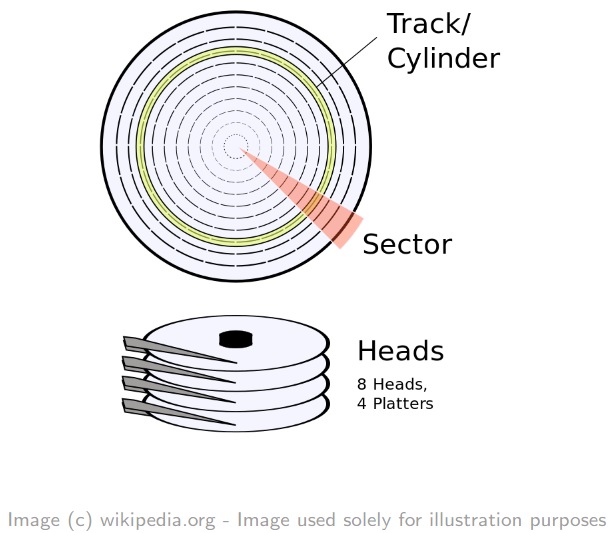
\includegraphics[scale=0.2]{images/chs.png}
        \captionsetup{labelformat=empty,labelsep=none}
        \transparent{0.4}%
        \caption[]{\tiny Image (c) wikipedia.org - Image used solely for illustration purposes}
    \end{figure}
\end{frame}


\begin{frame}[fragile]
  \frametitle{5.3 Low-Level: Sector Structur}
    \begin{figure}
        \includegraphics[scale=0.5]{images/sector.png}
        \captionsetup{labelformat=empty,labelsep=none}
        \transparent{0.4}%
        \caption[]{\tiny Image (c) forensicfocus.com - Image used solely for illustration purposes}
    \end{figure}
\end{frame}


\begin{frame}[fragile]
  \frametitle{5.4 Low-Level: Legacy considerations}
    \begin{itemize}
        \item[] Interleave Factor:
\begin{lstlisting}[basicstyle=\tiny]
Interleave factor 1:1 --> 01 02 03 04 05 06 07 08 09 10 11 12 13 14 15 16 17 
Interleave factor 2:1 --> 01 10 02 11 03 12 04 13 05 14 06 15 07 16 08 17 09 
Interleave factor 3:1 --> 01 07 13 02 08 14 03 09 15 04 10 16 05 11 17 06 12
\end{lstlisting}
        \item[] Zone Bit Recording:
\begin{lstlisting}[basicstyle=\tiny]
   Zone:  12  11  10  09  08  07  06  05  04  03  02  01  00
------------------------------------------------------------
 Tracks: 100 120 140 155 170 185 195 205 210 210 215 218 220
Sectors: 132 132 132 132 132 132 132 132 100 100 100 100 100
------------------------------------------------------------
\end{lstlisting}
        \item[] Head and Cylinder Skewing:
\begin{lstlisting}[basicstyle=\tiny]
No skewing
-----------
Cylinder 0: Head 0: |01 02 03 04 05 06 07 08 09 10 11 12 13 14 15 16 17
	    Head 1: |01 02 03 04 05 06 07 08 09 10 11 12 13 14 15 16 17
Cylinder 1: Head 0: |01 02 03 04 05 06 07 08 09 10 11 12 13 14 15 16 17

Head skew = 1, Cylinder skew = 4
--------------------------------
Cylinder 0: Head 0: |01 02 03 04 05 06 07 08 09 10 11 12 13 14 15 16 17
	    Head 1:  17|01 02 03 04 05 06 07 08 09 10 11 12 13 14 15 16
Cylinder 1: Head 0:  13 14 15 16 17|01 02 03 04 05 06 07 08 09 10 11 12
\end{lstlisting}
    \end{itemize}
\end{frame}


\begin{frame}[fragile]
  \frametitle{5.5 LBA - Logical Block Addressing - Abstract}
  \begin{lstlisting}[basicstyle=\tiny\ttfamily]
Logical volume addresses
----------------------------------------------------------------------------
|  0 |  1 |  2 |  3 |  4 |  5 |  6 |  7 |  8 |  9 | 10 | 11 | 12 | 13 | 14 |
----------------------------------------------------------------------------
          |                   |                   |                   |
          |                   |                   |                   |
          -------------------------------------------------------------
   ^      |         0         |         1         |         3         |   ^
   |      -------------------------------------------------------------   |
   |      Logical file system addresses - Clusters                        |
  MBR                                                               Volume slack
          *-------------------*
               2.048 Bytes
          *-----------------------------------------------------------*
                                   6.144 Bytes
  \end{lstlisting}
\end{frame}


\begin{frame}[fragile]
  \frametitle{5.6 MBR - Master Boot Record}
  \begin{lstlisting}[basicstyle=\tiny]
# dd if=/dev/sdc bs=512 count=1 skip=0 |xxd

0000000: fab8 0010 8ed0 bc00 b0b8 0000 8ed8 8ec0  ................
0000016: fbbe 007c bf00 06b9 0002 f3a4 ea21 0600  ...|.........!..
0000032: 00be be07 3804 750b 83c6 1081 fefe 0775  ....8.u........u
0000048: f3eb 16b4 02b0 01bb 007c b280 8a74 018b  .........|...t..
0000064: 4c02 cd13 ea00 7c00 00eb fe00 0000 0000  L.....|.........
0000080: 0000 0000 0000 0000 0000 0000 0000 0000  ................
0000096: 0000 0000 0000 0000 0000 0000 0000 0000  ................
...
...
0000432: 0000 0000 0000 0000 9af0 0200 0000 0020  ............... 
0000448: 2100 0b1b 0299 0008 0000 0080 2500 00a8  !...........%...
0000464: 01a8 071a b327 0058 2900 00c0 5d00 001a  .....'.X)...]...
0000480: b427 076c dad2 0018 8700 00c0 6800 0000  .'.l........h...
0000496: 0000 0000 0000 0000 0000 0000 0000 55aa  ..............U.



000 - 439       0x000 - 0x1B7    Boot code
440 - 443       0x1B8 - 0x1BB    Disc signature
444 - 445       0x1BC - 0x1BD    Reserved
446 - 509       0x1BE - 0x1FD    Partitiontable
510 - 511       0x1FE - 0x1FF    0x55 0xAA
  \end{lstlisting}
\end{frame}


\begin{frame}[fragile]
  \frametitle{5.6 MBR - DOS Partition Table}
  \begin{lstlisting}[basicstyle=\tiny,escapechar=\*]
# dd if=/dev/sdc bs=512 count=1 skip=0 |xxd

0000000: fab8 0010 8ed0 bc00 b0b8 0000 8ed8 8ec0  ................
0000016: fbbe 007c bf00 06b9 0002 f3a4 ea21 0600  ...|.........!..
0000032: 00be be07 3804 750b 83c6 1081 fefe 0775  ....8.u........u
0000048: f3eb 16b4 02b0 01bb 007c b280 8a74 018b  .........|...t..
0000064: 4c02 cd13 ea00 7c00 00eb fe00 0000 0000  L.....|.........
0000080: 0000 0000 0000 0000 0000 0000 0000 0000  ................
0000096: 0000 0000 0000 0000 0000 0000 0000 0000  ................
...
...
0000432: 0000 0000 0000 0000 9af0 0200 0000 *\underline{0020}*  ............... 
0000448: 2100 0b1b 0299 0008 0000 0080 2500 *\underline{00a8}*  !...........%...
0000464: 01a8 071a b327 0058 2900 00c0 5d00 *\underline{001a}*  .....'.X)...]...
0000480: b427 076c dad2 0018 8700 00c0 6800 *\underline{0000}*  .'.l........h...
0000496: 0000 0000 0000 0000 0000 0000 0000 55aa  ..............U.



Partitiontable:
  Offset: 0     Size: 1	Value: 0x80     --> Bootable
  Offset: 1     Size: 3	Value:          --> Starting CHS address
  Offset: 4     Size: 1	Value: 0x0b     --> FAT32
                               0x07     --> NTFS
  Offset: 5     Size: 3	Value:          --> Ending CHS address
  Offset: 8     Size: 4 Value:          --> Starting LBA address
  Offset:12     Size: 4 Value:          --> LBA size in sectors

  \end{lstlisting}
\end{frame}


\begin{frame}[fragile]
  \frametitle{5.6 MBR - DOS Partition Table}
  \begin{lstlisting}[basicstyle=\tiny,escapechar=\?]
  0000432: 0000 0000 0000 ?\texttt{0000 9af0}? ?\texttt{0200 0000}? 0020  ............... 
  0000448: 2100 0b1b 0299 ?\underline{0008 0000}? ?\underline{0080 2500}? 00a8  !...........%...
  0000464: 01a8 071a b327 ?\underline{0058 2900}? ?\underline{00c0 5d00}? 001a  .....'.X)...]...
  0000480: b427 076c dad2 ?\underline{0018 8700}? ?\underline{00c0 6800}? 0000  .'.l........h...
  0000496: 0000 0000 0000 ?\underline{0000 0000}? ?\underline{0000 0000}? 55aa  ..............U.

Partitiontable:
  Offset: 0     Size: 1	Value: 0x80     --> Bootable
  Offset: 1     Size: 3	Value:          --> Starting CHS address
  Offset: 4     Size: 1	Value: 0x0b     --> FAT32
                               0x07     --> NTFS
  Offset: 5     Size: 3	Value:          --> Ending CHS address
  Offset: 8     Size: 4 Value:          --> Starting LBA address
  Offset:12     Size: 4 Value:          --> LBA size in sectors
  
Addressable space:
  CHS: echo $((2^8 x 2^6 x 2^10 * 512 / 1024^2))  ==  8192 MByte
  LBA: echo $((2^32 * 512 / 1024^3))              ==     2 TByte
  \end{lstlisting}
    \begin{itemize}
	    \item[] Exercise: Calculate the size of the partitions
        \begin{enumerate}
            \item Take 4 byte from "LBA size"
	    \item Switch Little Endian value into Big Endian
	    \item Don't forget: Now you have the sector value, not the byte value
        \end{enumerate}
    \end{itemize}
\end{frame}


\begin{frame}[fragile]
  \frametitle{5.6 MBR - DOS Partition Table}
  \begin{lstlisting}[basicstyle=\tiny,escapechar=\?]
  0000432: 0000 0000 0000 ?\texttt{0000 9af0}? ?\texttt{0200 0000}? 0020  ............... 
  0000448: 2100 0b1b 0299 ?\underline{0008 0000}? ?\underline{0080 2500}? 00a8  !...........%...
  0000464: 01a8 071a b327 ?\underline{0058 2900}? ?\underline{00c0 5d00}? 001a  .....'.X)...]...
  0000480: b427 076c dad2 ?\underline{0018 8700}? ?\underline{00c0 6800}? 0000  .'.l........h...
  0000496: 0000 0000 0000 ?\underline{0000 0000}? ?\underline{0000 0000}? 55aa  ..............U.

  \end{lstlisting}
    \begin{itemize}
	    \item[] Exercise: Calculate the size if the partitions
    \end{itemize}
  \begin{lstlisting}[basicstyle=\tiny]
        Little Endian  Big Endian     Decimal     Sector size
-----------------------------------------------------------------------------
Part1:  0x00802500     0x00258000     2457600     * 512     1258291200   1.2 GB
Part2:  0x00c05d00     0x005dc000     6144000     * 512     3145728000   3.0 GB
Part3:  0x00c06800     0x0068c000     6864896     * 512     3514826752   3.4 GB
  \end{lstlisting}
    \begin{itemize}
        \item Demo:     Change partition type with hexeditor
	\item[] \texttt{fdisk -l /dev/sdb; hexedit /dev/sdb; F2, CTRL+x}
	\item[]
        \item Exercise: Find password in unused space before first partition
    \end{itemize}
\end{frame}


\begin{frame}[fragile]
  \frametitle{5.7 EBR - Extended Partitions}
  \begin{lstlisting}[basicstyle=\tiny]
MBR:  000001b0: 0000 0000 0000 0000 d7b8 0cae 0000 0014
      000001c0: 0904 050f 823e 0008 0000 0000 0400 0000


                           Extended Partition Container                          
------------------------------------------------------------------------------------
|EBR|000|     Logical     |                                                        |
------------------------------------------------------------------------------------
    --->                  ---------------------------
    --------------------> |EBR|000|     Logical     |
    Extended Partition    ---------------------------
                              --->                  ---------------------
    ----------------------------------------------> |EBR|000|  Logical  |
                              Extended Partition    ---------------------
                                                        --->

EBR_01:  001001b0: 0000 0000 0000 0000 0000 0000 0000 0029
         001001c0: 0708 0717 0a2c 0008 0000 0040 0000 0018
         001001d0: 012c 051f 4206 0048 0000 0088 0100 0000

         EBR_02:  00A001B0: 0000 0000 0000 0000 0000 0000 0000 002C
                  00A001C0: 0930 071F 4206 0008 0000 0080 0100 001F
                  00A001D0: 4306 0503 8228 00D0 0100 0008 0200 0000

                  EBR_03:  03B001B0: 0000 0000 0000 0000 0000 0000 0000 0006
                           03B001C0: 410B 0703 8228 0008 0000 0000 0200 0000
                           03B001D0: 0000 0000 0000 0000 0000 0000 0000 0000
  \end{lstlisting}
\end{frame}


\begin{frame}[fragile]
  \frametitle{5.8 GPT - GUID Partition Table}
    \begin{itemize}
        \item BIOS $\to$ UEFI - Unified Extensible Firmware Interface
	\item GUID - Globally Unique Identifier for each partition
	\item[] $\to$ GUID Partition Table
	\item Protective MBR at LBA0
        \begin{itemize}
            \item One single entry covering the entire disk
            \item Partition type 0xEE
	    \item[] if 0xEE unknown $\to$ Not empty $\to$ Not formatted
        \end{itemize}
	\item GPT header at LBA1
	\item GPT entries at LBA2 $\to$ LBA34
	\item GPT entries: 128 Bytes
	\item GPT backup at end of disk
    \end{itemize}
\end{frame}


\begin{frame}[fragile]
  \frametitle{5.8 GPT - GUID Partition Table}
    \begin{figure}
        \caption[]{\tiny Image (c) wikipedia.org - Image used solely for illustration purposes}
	    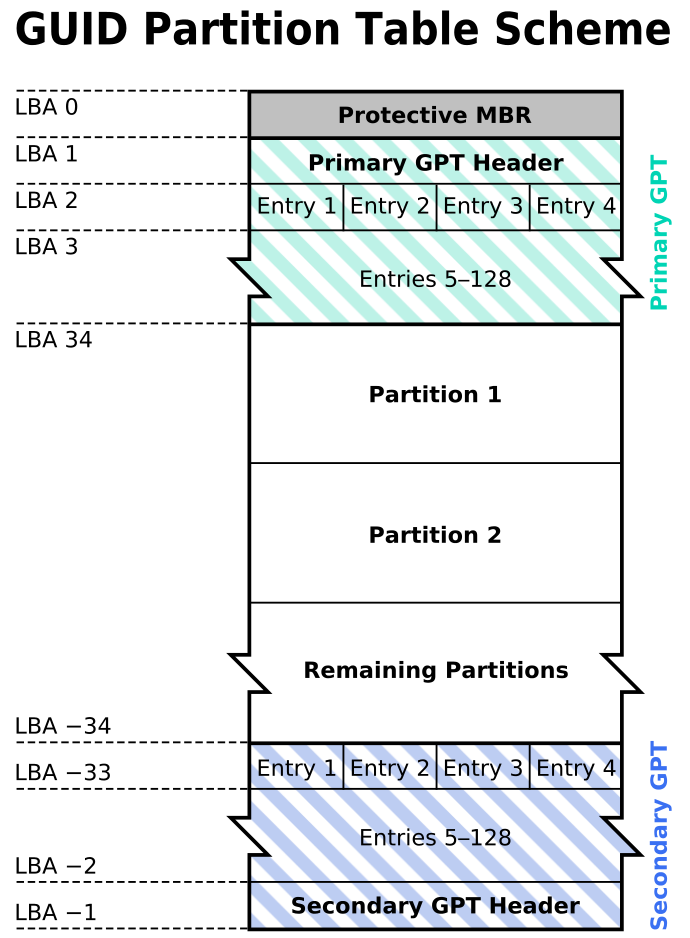
\includegraphics[scale=0.23,angle=270]{images/gpt.png}
        \captionsetup{labelformat=empty,labelsep=none}
        \transparent{0.4}%
    \end{figure}
\end{frame}


\begin{frame}[fragile]
  \frametitle{5.9 VBR - Volume Boot Record - Boot Sector}
  \begin{lstlisting}[basicstyle=\tiny]
# dd if=/dev/sdc1 bs=512 count=1 skip=0 |xxd

0000000: eb58 906d 6b64 6f73 6673 0000 0208 2000  .X.mkdosfs.... .     # 0xeb 0x58 0x90
0000010: 0200 0000 00f8 0000 3e00 f800 0000 0000  ........>.......     # JMP  2+88 NOP
0000030: 0100 0600 0000 0000 0000 0000 0000 0000  ................
0000040: 0000 29a2 20e9 9c46 4154 2020 2020 2020  ..). ..FAT      
0000050: 2020 4641 5433 3220 2020 0e1f be77 7cac    FAT32   ...w|.
0000060: 22c0 740b 56b4 0ebb 0700 cd10 5eeb f032  ".t.V.......^..2
...
...
00001f0: 0000 0000 0000 0000 0000 0000 0000 55aa  ..............U.


0 - 2           Size:  3    Jump to bootstrap code
3 - 10          Size:  8    OEM-ID: mkdosfs
11 - 12         Size:  2    Bytes per sector: 0x0002 -> 0x0200 (little endian)-> 512
13 (0xD)        Size:  1    Sectors per cluster: 0x08 -> 4096 bytes per cluster
50 (0x32) - 51  Size:  2    Boot sector backup: 0x0600 -> 0x0006 -> at sector 6
67 (0x43) - 70  Size:  4    Volume serial number: 0xa220e99c -> 0x9ce920a2
71 (0x47)       Size: 11    Volume label: FAT
82 (0x52)       Size:  8    Partition type: FAT32
90 (0x5A)- 509 (0x1FD)	    Bootstrap code
510 (0x1FE)     Size:  2    Signature: 0x55AA
  \end{lstlisting}
    \begin{itemize}
        \item Demo: Sleuthkit tools: \texttt{mmstat, mmls, fsstat}
    \end{itemize}
\end{frame}




